\section{Question 2} \label{sec:Q2}

\textit{\textbf{Calculate the NR value of the conference room.}}

The background noise in the conference room is due to the fan noise transmitted through the ductwork (both supply and return).
Hence, the SPLs calculated in Question~1 (see L\textsubscript{p\textsubscript{1}} in Table~\ref{tbl:BN_conf}) have been plotted on the noise rating (NR) curve chart.
%in Figure 2.
As seen in Figure~\ref{fig:NR_conf}, the SPLs lie on/ below the NR 50 curve.
Therefore, the conference room's noise rating is NR 50.

According to Table~2.5 in the course notes \citep{unit2}, the recommended NR for an office ranges between 25 and 45.
The conference room's NR of 50 can therefore be seen as a bit high.

\begin{figure}[htbp]
	\centering
	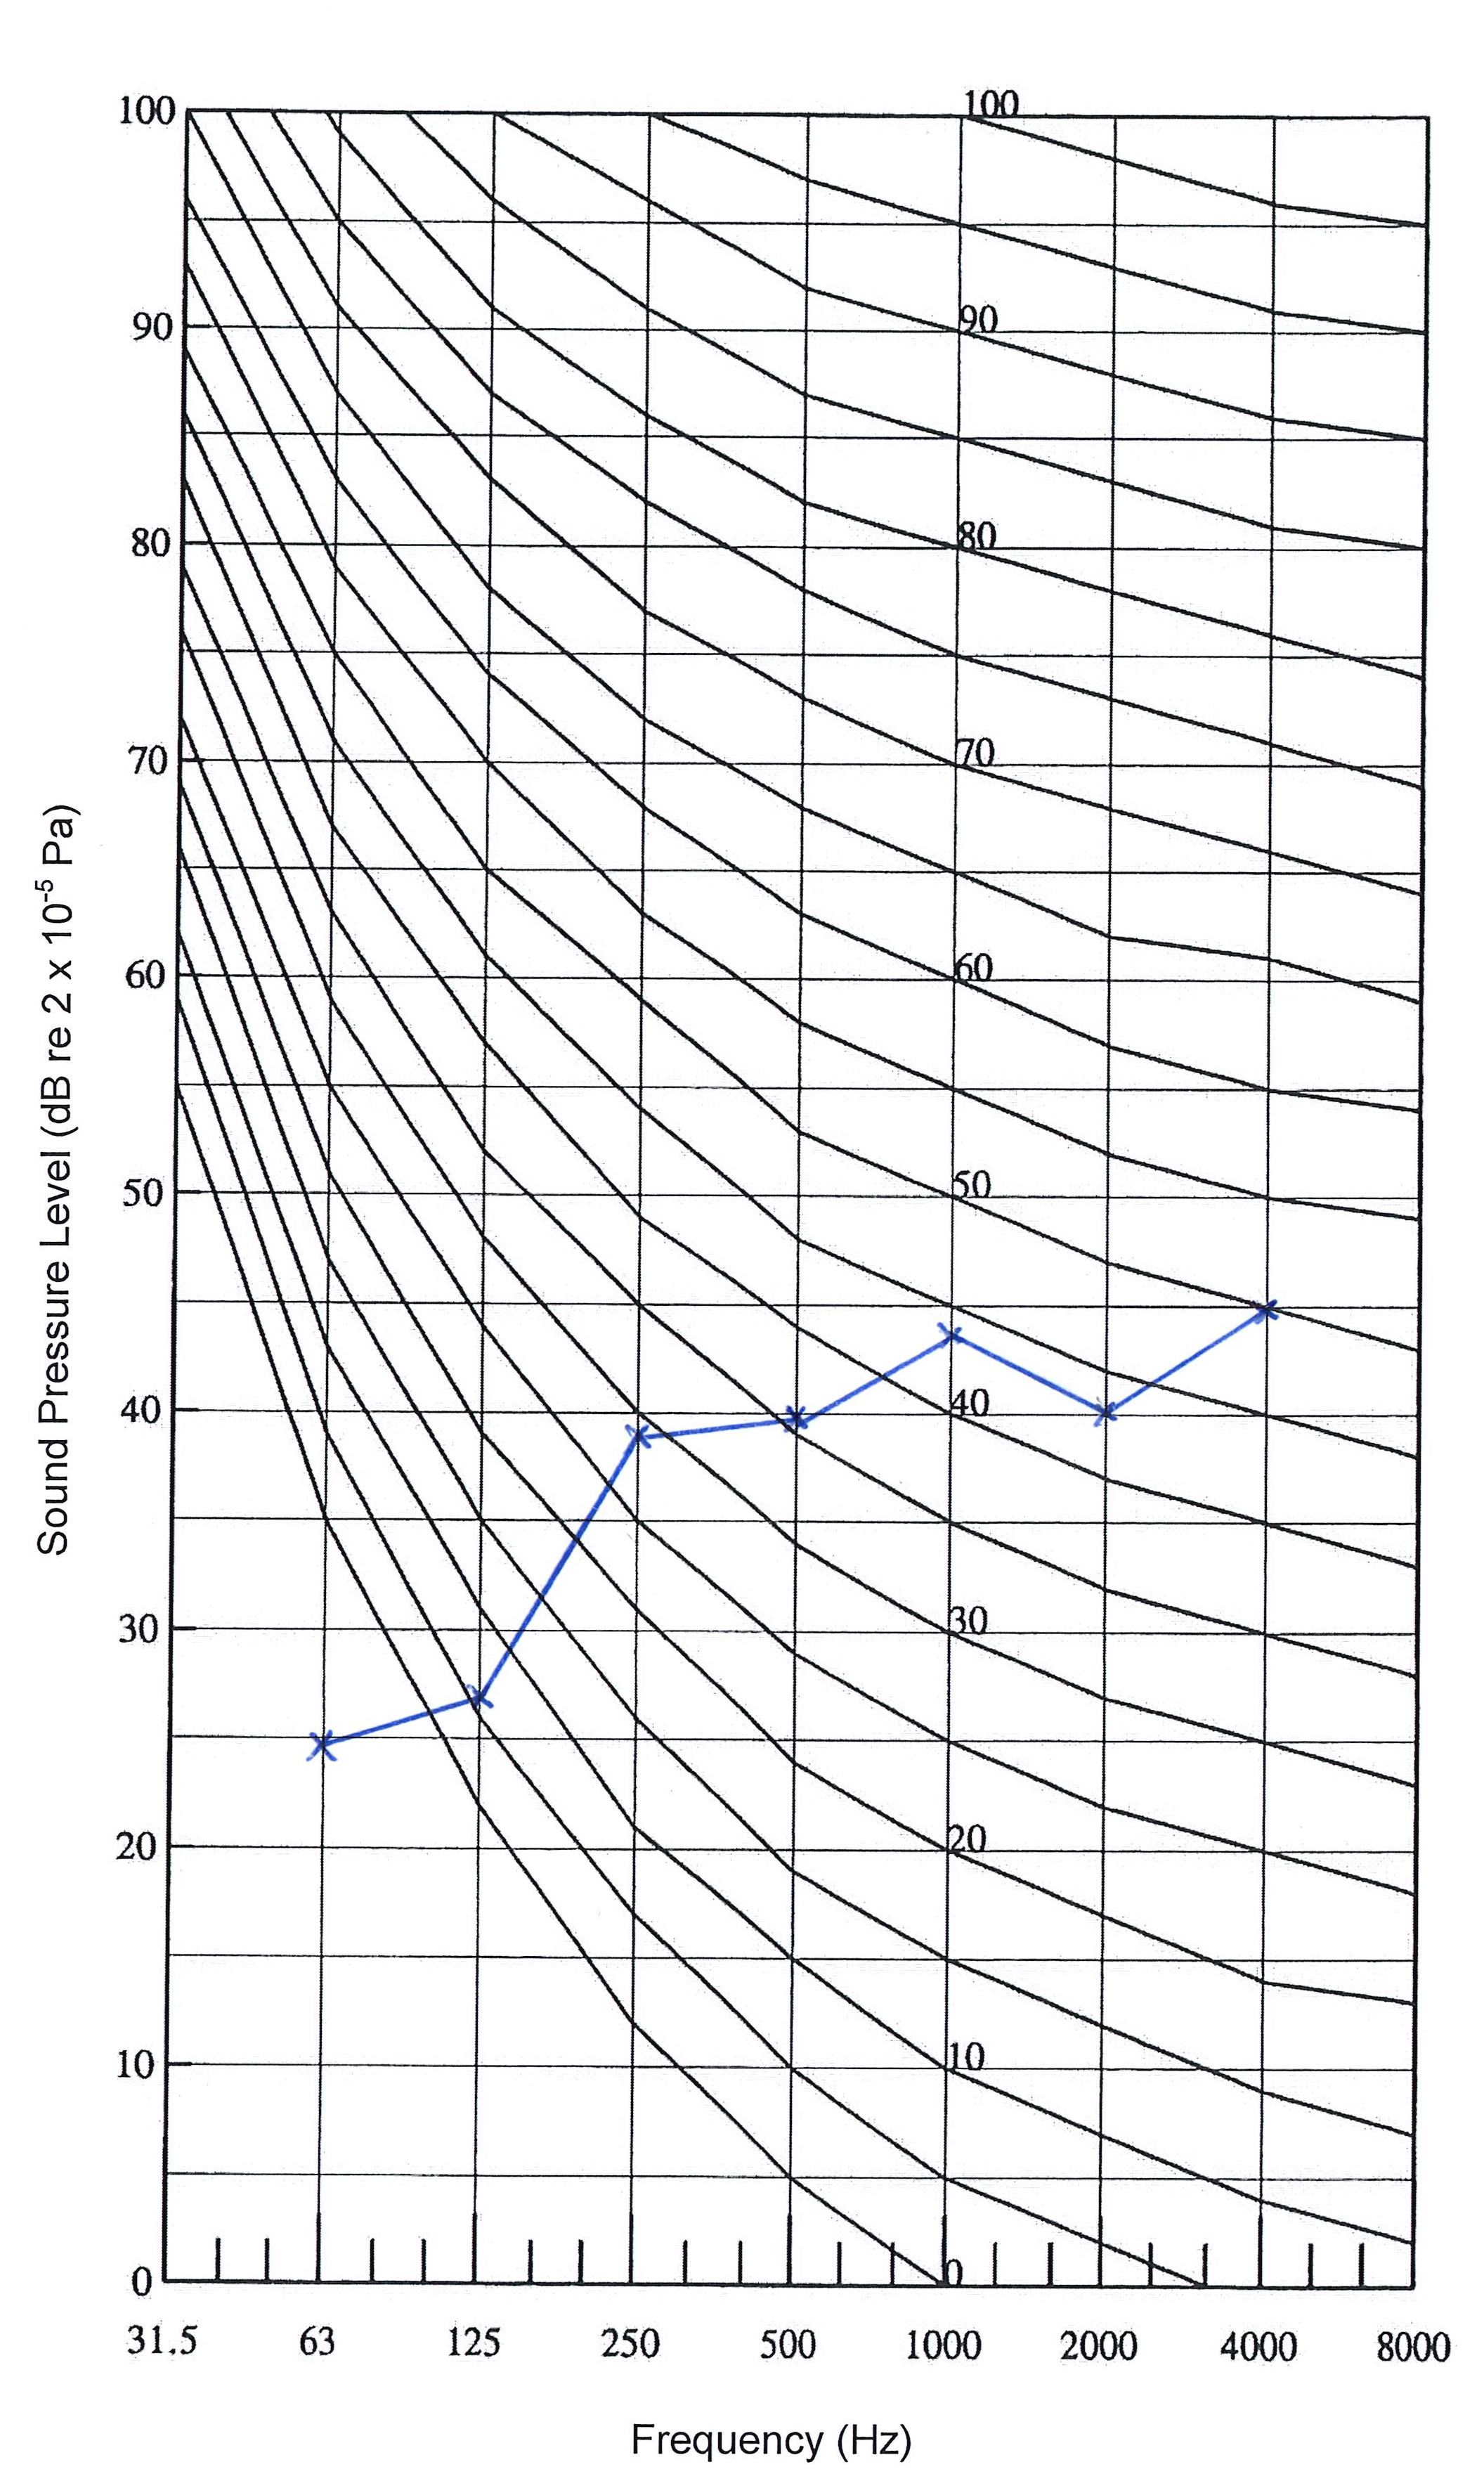
\includegraphics[height=.65\textheight]{figures/NR_conference.jpg}
	\rule{.6\textwidth}{0.5pt} % use line???
	\caption{The NR of the conference room.}
	\label{fig:NR_conf}
\end{figure}